\documentclass[index]{subfiles}

\begin{document}
\title{Chinese Remainder Theorem}
\date{}
\author{}
\maketitle

\newpage

\addtocontents{toc}{\protect\thispagestyle{empty}}
\tableofcontents
\thispagestyle{empty}
\newpage
\setcounter{page}{1}

\section{Introduction}

The water bottle problem has been a problem that I've come across multiple times throughout my life, ever since I was a child. I've seen it in multiple video games, as well as multiple math problems. Whenever I've come across these problems, I've admired the fact that just by ``messing around with it'', a solution that isn't obvious at first sight reveals itself. Through trial and error, these problems can always be solved. But there have always been times when I've tried those problems in the games and thought: would there be situations where the problem isn't solvable? What combinations of cups made the problems solvable? And, what if I didn't have an infinite amount of water to play around with in the first place? what would be the most optimal solutions?

When I first came across the Chinese Remainder Theorem, I knew that I had to explore this topic further because it answered all my questions and more.

\section{Initial Problem}

The initial problem is as follows: An unknown amount of water poured over and over into one container with a 3L capacity gives 1L left over, and over another container with a 5L capacity leaves 4L leftover, and finally, in a container with a 7L capacity gives 6L leftover. What is the original quality leftover?


\section{An exploration of modular arithmetic}

To approach this problem, modular arithmetic can be used. Modular arithmetic is simply a way to express remainders in a problem clearly. Take the simple expression of dividing a number, 5, by 2, for example. Before coming across modular arithmetic, if you wanted to express the results of this problem including the remainder, you might write it as

\begin{equation*}
    \frac{5}{2}=2\ remainder\ 1
\end{equation*}

Where 5 is the dividend, the 2 in the fraction is the divisor, the 2 as the result is the quotient, and finally 1 being the remainder.

However, what if you didn't care about what the whole number was, but just the amount that was left? You might revise the expression above to write it as

\begin{equation*}
    \frac{5}{2}=\dots remainder\ 1
\end{equation*}

One observation from this set of equations is that, since we only care about the remainder of the expression, expressions could have different operands, but still result in a remainder of 1, which we could then consider to be equal..

\begin{equation*}
    \frac{7}{2}=\frac{5}{2}=\dots remainder\ 1
\end{equation*}

Let's convert this expression to the official way to express this, creating what is known as a congruence statement.

\begin{equation*}
    5\equiv 1 \mod 2
\end{equation*}

This expression is read as ``5 is of the same congruence class as 1, mod 2''.

The \(1\) still stands for the remainder of the problem, when divided by \(2\). It's similar to a regular mathematical expression \(\frac{x}{2}=y (remainder\ 1)\), except there is no \(y\), that value is ignored.

Let's break down the notation of this equation, which includes two new symbols, \(\equiv\) and \(\mod\).


\(\mod x\) stands for ``modulo'' which denotes the euclidean remainder of a number. This operator is nonstandard in two ways. One is in its ordering. Instead of reading from left to right like a standard operator operating on an operand, it's instead in a non-linear order and exists on the right. Recall how the expression is read. Instead of saying that ``5 divided by 2 yields a remainder of 1'' as one might read regular division operations, the ordering of \(\mod\) places the remainder ahead of the quotient, such that the expression is read as ``5 is congruent to 1, mod 2''.

The second thing to know about this operator is that it doesn't simply describe an intuitive remainder between two numbers, rather, it describes the \textbf{euclidean remainder}. Euclidean remainder is almost the same as a `regular' remainder (that one receives from dividing a number using long division), except it treats negative numbers slightly different from regular remainders.
Euclidean division defined as follows:

If there is a divided \(a\) and a divisor \(b\), the relation between the two numbers can be defined as

\[a=bq+r\]

, where \(q\) is known as the quotient and

\[0\leq r<|b|\] and both \(q\) and \(r\) are entirely unique integers (\(q,r \in\mathbb{Z}\)). The key to note here is that with this definition, the remainder is always defined as a positive integer, which might lead to  different behavior than one would intuitively expect.

For example, one might expect to express the euclidean remainder of \(-13\) and \(6\) in \[\frac{-13}{6}\] in the form

\[-13=6\cdot-2+-1\]

but if we only want the remainder to be positive, then we would instead choose to distribute more negatives such that we could return a positive remainder

\[-13=6\cdot-3 + 5\]

This is an important distinction to make, one because it affects results later on, and second, because it helps explain the \(\equiv\) symbol.

The \(\equiv \) sign denotes that \(X\) is in the same congruence class as \(1\) when taken the modulo. What does it mean by congruence class? Well, think of all numbers that have a remainder of 1 when divided by 3. (khan academy). These are 1, 4, 7, 10, so on and so forth. When a number has the same remainder when divided by a number, they are in the same ``congruence class'' as each other. Therefore, the current equation that we have setup, while similar to a system of equations, because it has ``congruence'' statements along with modulo, is called a ``system of congruences'' instead of a system of equations.

\begin{figure}[H]
    \centering
    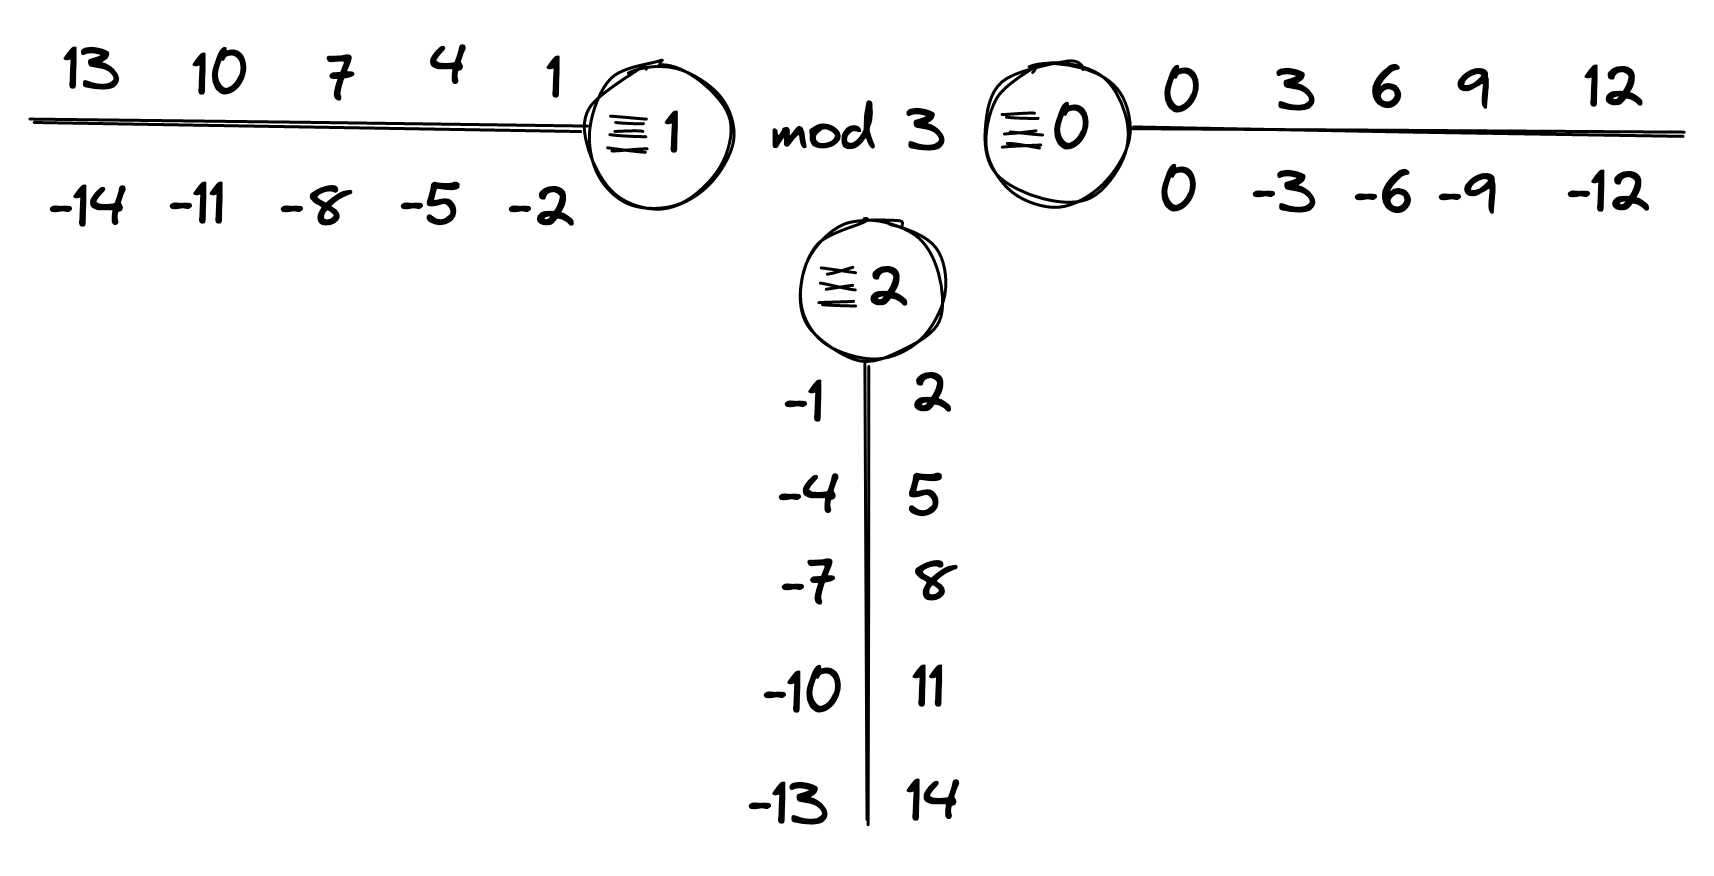
\includegraphics[scale=0.2]{pics/congruence_class.png}
    \caption{Visualization of congruence classes of 0, 1, and 2 for numbers \(\mod 3\), with inspiration from Khan Academy}
\end{figure}

With these explanations, we can rephrase the way that we see the water bottle problem. We call the total amount of water that we have \(X\). \(X\) amount of water can divided over a container of \(3L\) capacity some integer number of times, leaving behind \(1L\). Thus,

\begin{equation*}
    X\equiv1\mod3
\end{equation*}

We can repeat the same reasoning for the \(7L\) container leaving \(6L\) of water leftover, and the \(5L\) container leaving \(4L\) of water, and express them in terms of congruence statements.

Thus, combined, the above water problem can then be expressed as the following \textit{system of congruences}.

\begin{align*}
    X\equiv 1\mod 3 \\
    X\equiv 4\mod 5 \\
    X\equiv 6\mod 7 \\
\end{align*}

\section{The Chinese Remainder Theorem}

Here's where the Chinese Remainder Theorem comes into play. The way that we can solve a system of congruences in modular arithmetic is much different from how one solves a regular system of equations. Instead of substituting and using regular algebra, the conventional way to solve a system of congruences is using an entire theorem, the Chinese Remainder theorem. The Chinese Remainder Theorem states the following: Given a system of equations as defined as follows

\begin{align*}
    X & \equiv a_1\mod n_1 \\
    X & \equiv a_2\mod n_2 \\
      & \ldots
\end{align*}

Where \(n_x\) are coprime (meaning they don't have any common factors other than 1), or the \(gcf(m1, m2, \ldots)=1\), there is always a solution to this system, \(X\), where

\begin{equation*}
    X\equiv (a_1N_1N_1^{-1} + a_2N_2N_2^{-1} + \cdots + a_{n}N_{n}N_{n}^{-1})\mod N
\end{equation*}~\parencite{nesoacademyChineseRemainderTheorem2021}

We can slightly simplify the above expression and write it as a series, starting from \(1\) and ending at \(n\), the number of congruence statements we have inside the system. 

\begin{equation*}
    X\equiv \sum_{i=1}^{n}a_{i}N_{i}N_{i}^{-1}\mod N
\end{equation*}

\subsection{Breaking down the theorem}

While the above statement may seem complex, it simply boils down to finding the values for the unknown \(N\)s. There 2 unknowns per congruence statement, \(N_i\) and \(N_i^{-1}\) that must be solved for, as well as \(N\).

We can find \(N\) by multiplying each individual \(n_i\) in the system of equations together,

\begin{equation*}
    N=n_1\times n_2 \times \cdots \times n_i
\end{equation*}

The \(N_i\) for each individual congruence statement can then be calculated by dividing \(N\) by \(n_i\).

\begin{equation*}
    N_i=\frac{N}{n_i}
\end{equation*}

And finally, to find \(N_i^{-1}\) (also called the inverse of the modulo), we state that

\begin{equation*}
    N_i\cdot N_i^{-1}\equiv 1 \mod n_i
\end{equation*}

Then find \(N_i^{-1}\) by solving the congruence statement. This can be accomplished via simple guessing and checking, or by using Bézout's identity, which the coefficients can be calculated using Euclid's Extended algorithm.

Finally, after finding all the required values, we can then find \(X\) by plugging into the formula with known values of \(a_{i}, N_{i}, and\ N_{i}^{-1}\), then finding an \(X\) which is within the same congruence class as the resulting value.

\section{Working through the problem}

\subsection{The easy values}

Since \(N=n_1\times n_2\times\cdots\times n_n\), we simply multiply the capacities of the three containers together

\begin{align*}
    N&=3\cdot5\cdot7\\
    &=\boxed{105}
\end{align*}

Next we'll find \(N_1\), \(N_2\), and \(N_3\) by dividing the \(N\) we just found by each \(n_i\)

\begin{align*}
    N_1&=\frac{N}{n_1}\\
    &=\frac{105}{3}\\
    &=\boxed{35}\\
    N_2&=\frac{N}{n_2}\\
    &=\frac{105}{5}\\
    &=\boxed{21}\\
    N_3&=\frac{N}{n_3}\\
    &=\frac{105}{7}\\
    &=\boxed{15}\\
\end{align*}

\subsection{Calculating the inverse modulo}

Then here's where the hard part starts: we need to find \(N_1^{-1}\), \(N_2^{-2}\), and \(N_3^{-3}\), known as the modular multiplicative inverse, for each congruence statement, given that 

\begin{equation*}
    N_i\cdot N_i^{-1}=1\mod n_i
\end{equation*}

Let's start with \(i=1\), or the container with the capcity of \(3L\) first. Repacing \(i\) with \(1\), we would then have

\begin{equation*}
    N_1\cdot N_1^{-1}=1\mod n_1
\end{equation*}

We can easily plugin the values for \(N\) and \(n_1\), which we have already calcualted, yielding

\begin{equation*}
    35\cdot N_1^{-1}=1\mod 3
\end{equation*}

How do we then proceed from here? One way to continue is to use a method of brute force: by guessing and checking. We could try to set \(N_1^{-1}\) to random integers, such as \(1, 2, 3,\cdots\), and see if the euclidean remainder of \(35\cdot N_1^{-1}\) and \(3\) becomes \(1\). While this is a valid way to approach this, it is obviously not very efficient, and should the problem even have slightly larger numbers, it would take many iterations to reach the correct answer. Thus, to solve for the multiplicative inverse, a more systematic method will be used, as mentioned earlier, using Bézout's identity and the Extended Euclid Algorithm. The following sections will be dedicated to explaining what they are as well as the basic proof for Euclid's Algortithm.

\subsection{Eulid's Algorithm}

Euclid's algorithm is a method of easily and efficiently calcualting the greatest common factor (also referred to as greatest common demoninator, \(\gcd\)) between two numbers.

It's based on the idea that given two numbers \(A\) and \(B\) where \(A, B \in \mathbb{Z}\) (they're both real numbers) and \(B\) is the smaller number (\(B\leq A\)), the greatest common factor of two numbers is equal to the greatest common factor between \(A\) and \(B\)

\[\gcd(A,B)=\gcd(B, A-B)\]

Thus the greatest common factor can be found by putting putting equations in the form of the euclidean division form, \(a=bq+r\).

\begin{align*}
    a & =bq+r   \\
    b & =rq+r_1 \\
      & \ldots  \\
    r & =r_1q+0
\end{align*}

With the ending divisor, \(r_1\) as the \(\gcd(a, b)\).

\subsubsection{Euclid's Algorithm Example}

Say we wish to find the greatest common factor between \(7\cdot11=77\) and \(7\cdot18=126\). First we would lay it out in the form \(a=bq+r\)

\begin{align*}
    126 & =77q+r
    \intertext{Then we would use long division to find that 77 only goes into 126 one time, and thus the remainder is simply \(126-77(1)=49\)}
    126 & =77(1)+49
    \intertext{We would then replace the dividend, 126, by the divisor, 77, and replace 77, the divisor, by the remainder, 49}
    77  & =49(1)+28
    \intertext{We repeat this process until we reach a remainder of 0}
    49  & =28(1)+21 \\
    28  & =21(1)+7  \\
    21  & =7(3)+0
\end{align*}

And 7 is the dividend where the remainder equals 0, thus 7 divides 77 and 126 evenly and thus \(\gcd(77, 126)\) is equal to 7.

\subsection{Euclid's Algorithm Proof}

Because of the use of Euclid's Algorithm as a foundational principle for solving modular arithmetic in its application to the chinese remainder theorem, a proof is definitely called for. Though, the proof for Euclid's Algorithm is rather intuitive and can be visualized easily.

Again, we are given \(A, B \in \mathbb{Z}\), and we wish to find the \(\gcd\) between the two numbers.

First of all, we can prove the base case fairly easily. If \(A=0\), then \(\gcd(A,B)=B\), since any number can be divided 0 times evenly (i.e., \(B\cdot0=A\)). Similarly, if \(B=0\), then \(\gcd(A,B)=A\).

\subsubsection{\texorpdfstring{Next, we prove that \(\gcd(A,B)\) divides \(C\), the difference between \(A\) and \(B\), evenly.}{Lg}}

\begin{align*}
    \intertext{To start, we express the relationship between \(A\), \(B\), and \(C\) in an equation}
    A-B                   & =C \\
    \intertext{Next, we know that by definition, \(\gcd(A,B)\) evenly divides \(A\) by a factor, which we'll call \(X\), where \(X\in\mathbb{Z}\)}
    X\gcd(A,B)            & =A \\
    \intertext{By the same line of reasoning, \(\gcd(A,B)\) evenly divides \(B\) by a factor, which we can call \(Y\), where \(Y\in\mathbb{Z}\)}
    Y\gcd(A,B)            & =B \\
    \intertext{Substituting \(A\) and \(B\) in terms of the \(\gcd(A,B)\) into the original relationship yields}
    X\gcd(A,B)-Y\gcd(A,B) & =C
    \intertext{Where the \(\gcd\) can be factored out to yield}
    (\gcd(A,B))(X-Y)      & =C
\end{align*}

Since \(X,Y\in\mathbb{Z}\), \(X-Y\) must also be an integer, so we have proved that \(\gcd(A,B)\) evenly divides \(C\).

\subsubsection{\texorpdfstring{Next, we prove that \(\gcd(B,C)\) divides \(A\) evenly}{Lg}}

\begin{align}
    \intertext{To start, we express the relationship between \(A\), \(B\), and \(C\) in an equation}
    A-B        & =C                       \\
    A          & =B+C                     \\
    \intertext{Next, we know that by definition, \(\gcd(B,C)\) evenly divides \(B\) by some integer factor which we'll call \(X\)}
    X\gcd(B,C) & =B                       \\
    \intertext{By the same method of reasoning, we know that by definition, \(\gcd(B,C)\) evenly divides \(C\) by some integer factor which we'll call \(Y\)}
    Y\gcd(B,C) & =C                       \\
    \intertext{Then we substitute the values of \(B\) and \(C\) in terms of \(\gcd(B,C)\) back into the relationship equation}
    A          & =X\gcd(B,C) + Y\gcd(B,C) \\
    A          & =(\gcd(B,C))(X+Y)
\end{align}

And since \(X,Y\in\mathbb{Z}\), \(X+Y\) must also be an integer, so we have proved that \(\gcd(B,C)\) evenly divides \(A\).

\subsubsection{\texorpdfstring{Proving that \(\gcd(A,B)=\gcd(A, A-B)\)}{Lg}}

The core part of the Euclidean Algorithm is that the greatest common denominator of two numbers is also the greatest common denominator of their difference, and thus the following section makes up the core of the proof.

Now to summarize what we have so far, we know that as \(\gcd(A,B)\) evenly divides into \(C\), the \(\gcd(A,B)\) is then a factor of \(A,B,C\). Then as \(\gcd(B,C)\) evenly divides into \(A\), the \(\gcd(B,C)\) is then also a factor of \(A,B,C\).

But then,

\begin{align*}
    \gcd(A,B)   & \leq\gcd(B,C)
    \intertext{since by the definition of \(\gcd\), \(\gcd(B,C)\) is the \textbf{greatest} factor of both \(B,C\)}
    \gcd(B,C)   & \leq\gcd(A,B)
    \intertext{since by the definition of \(\gcd\), \(\gcd(A,B)\) is the \textbf{greatest} factor of both \(A,B\). Then by a transitive property of sorts,}
    \gcd(A,B)   & =\gcd(B,C)
    \intertext{and by definition the difference \(C=A-B\), so}
    \gcd(A,B)   & =\gcd(B,A-B)
    \intertext{From there, it's a simple matter of rearranging and simplifying terms.}
    \gcd(B,A-B) & =\gcd(A-B,B)
    \intertext{Then, we can apply recursion to the rule. If we think of \(A-B\) as the new \(A\) in \(\gcd(A,B)=\gcd(A-B,B)\), then it follows that}
    \gcd(A,B)=\gcd(A-B,B)=\gcd(A-2B,B)&=\gcd(A-3B,B)\ldots\gcd(A-BQ,B)
    \intertext{But from euclidean division, we know that}
    A           & =BQ+R         \\
    R           & =A-BQ
    \intertext{Thus, substituting that into the recursed result, we get}
    \gcd(A,B)   & =\gcd(A-BQ,B) \\
    \gcd(A,B)   & =\gcd(R,B)
\end{align*}

As an extension to the above Eulid's Algorithm is Bézout's Identity, a thoerem which assets that given two integers with a common factor \(D\) (i.e. \(A,B\in\mathbb{Z}\) and \(\gcd(A,B)=D\)), their relationship can be expressed in the form 

\begin{equation*}
    AX+BY=D
\end{equation*}

Where \(X,Y\in\mathbb{Z}\).

This is especially useful if we wish to calculate the multiplicative inverse \(N^{-1}\) as required by the Chinese Remainder Theorem, since if the \(\gcd(A,B)=1\), and \(A\) and \(B\) are coprime, then 

\begin{equation*}
    AX+BY=1
\end{equation*}

The coefficients \(A\) and \(B\) can be found using Euclid's Extended algorihtm, which, as the name suggest, it's an extension of Euclid's Algorithm with a few extra steps.

\subsection{Application of Euclid's Algorithm and Bézout's Identity}

To return back to where we left off, the Chinese Remainder Theorem by definition requires the quotients of the system of congruences (\(n_1\), \(n_2\), and \(n_3\)) to be coprime. For this system of congruences that we formed to represent the water battle problem, this is the case, since \(\gcd(3,5)=\gcd(5,7)=\gcd(3,7)=1\), it follows that for any system of congruence in this problem, \(\gcd(N_i,n_i)=1\). We can also validate this by taking the modified congruence statement that includes the modular multiplicative inverse

\begin{equation*}
    35\cdot
\end{equation*}

and seeing that \(\gcd()\)

\newpage

\raggedright{}
\printbibliography[heading=bibintoc]

\end{document}